% Template for ICIP-2018 paper; to be used with:
%          spconf.sty  - ICASSP/ICIP LaTeX style file, and
%          IEEEbib.bst - IEEE bibliography style file.
% --------------------------------------------------------------------------
\documentclass{article}
\usepackage{spconf,amsmath,graphicx}
\usepackage{amsthm}
\usepackage{hyperref}
\usepackage{algorithm}
\usepackage[noend]{algpseudocode}
\usepackage{etoolbox}
\usepackage{xcolor}

% Algorithmic gray vertical lines
\definecolor{lgray}{gray}{0.75}
\makeatletter
% start with some helper code
% This is the vertical rule that is inserted
\newcommand*{\algrule}[1][\algorithmicindent]{%
  \makebox[#1][l]{%
    \color{lgray}
    \hspace*{.2em}% <------------- This is where the rule starts from
    \vrule height .75\baselineskip depth .25\baselineskip
  }
}

\newcount\ALG@printindent@tempcnta
\def\ALG@printindent{%
    \ifnum \theALG@nested>0% is there anything to print
    \ifx\ALG@text\ALG@x@notext% is this an end group without any text?
    % do nothing
    \else
    \unskip
    % draw a rule for each indent level
    \ALG@printindent@tempcnta=1
    \loop
    \algrule[\csname ALG@ind@\the\ALG@printindent@tempcnta\endcsname]%
    \advance \ALG@printindent@tempcnta 1
    \ifnum \ALG@printindent@tempcnta<\numexpr\theALG@nested+1\relax
    \repeat
    \fi
    \fi
}
% the following line injects our new indent handling code in place of the default spacing
\patchcmd{\ALG@doentity}{\noindent\hskip\ALG@tlm}{\ALG@printindent}{}{\errmessage{failed to patch}}
\patchcmd{\ALG@doentity}{\item[]\nointerlineskip}{}{}{} % no spurious vertical space
% end vertical rule patch for algorithmicx
\makeatother

\newtheorem{definition}{Definition}
\newtheorem{theorem}{Theorem}
\newtheorem{proposition}{Proposition}
\newtheorem{corollary}{Corollary}
\newtheorem{lemma}{Lemma}
\newtheorem{exercise}{Exercise}
\newtheorem{example}{Example}

\DeclareMathOperator*{\argmin}{arg\,min}
\DeclareMathOperator*{\argmax}{arg\,max}
\DeclareMathOperator*{\Val}{\text{Val}}
\DeclareMathOperator*{\Ch}{\text{Ch}}
\DeclareMathOperator*{\Pa}{\text{Pa}}
\DeclareMathOperator*{\Sc}{\text{Sc}}
\newcommand{\ov}{\overline}
\newcommand{\tsup}{\textsuperscript}

\newcommand{\algorithmautorefname}{Algorithm}
\algrenewcommand\algorithmicrequire{\textbf{Input}}
\algrenewcommand\algorithmicensure{\textbf{Output}}

% Example definitions.
% --------------------
\def\x{{\mathbf x}}
\def\L{{\cal L}}

% Title.
% ------
\title{VISUALIZING GENERATIVE SUM-PRODUCT NETWORKS ON IMAGE RECONSTRUCTION}
% Single address.
% ---------------
\name{Renato L. Geh}
\address{University of São Paulo\\Institute of Mathematics and Statistics\\
  Rua do Matão, 1010 - São Paulo, SP, Brazil, 05508-090}
%
% For example:
% ------------
%\address{School\\
%	Department\\
%	Address}
%
% Two addresses (uncomment and modify for two-address case).
% ----------------------------------------------------------
%\twoauthors
%  {A. Author-one, B. Author-two\sthanks{Thanks to XYZ agency for funding.}}
%	{School A-B\\
%	Department A-B\\
%	Address A-B}
%  {C. Author-three, D. Author-four\sthanks{The fourth author performed the work
%	while at ...}}
%	{School C-D\\
%	Department C-D\\
%	Address C-D}
%
\begin{document}
%\ninept
%
\maketitle
%
\begin{abstract}
  Sum-Product Networks (SPNs) are fairly recent deep tractable probabilistic graphical models that
  are able to answer exact queries in linear time. Although there have been many advancements in
  practical problems, there is an absence in literature of visualizations on how SPNs represent
  learned data. In this paper we show how two structure learning algorithms can heavily impact on
  how SPNs treat data, particularly in the domain of image reconstruction. We show a coloring
  technique to visualize sum and product nodes through their scopes. We then apply this technique
  to generative SPNs learned from two distinct learning methods.
\end{abstract}
%
\begin{keywords}
Sum-product networks, probabilistic graphical models, visualization, image reconstruction
\end{keywords}
%
\section{Introduction}
\label{sec:intro}

Image reconstruction is the task of accurately predicting, guessing and completing missing elements
from an image. Density estimators that model a joint probability distribution can achieve this by
learning the features of similar images and finding the valuation that most adequately fits the
incomplete image. However, classical density estimators, such as Probabilistic Graphical Models
(PGMs), suffer from exact inference intractability in the general case. This leads to approximate
prediction and representation, as learning in PGMs often requires the use of inference as a
subroutine.

Sum-Product Networks (SPNs)~\cite{poon11} are fairly recent tractable PGMs capable of representing
distributions as a deep network of sums and products. Most importantly, SPNs are capable of exact
inference in time linear to its graph's edges. There have been many advances on SPNs in the image
domain, such as image classification and reconstruction~\cite{gens13,dennis12,gens12}, image
segmentation~\cite{yuan16} and activity recognition~\cite{amer12,amer16,wang18}. However, there
have been little effort~\cite{vergari16} so far to explore SPNs' semantics and representation
power.

In this paper, we provide visualizations on SPNs learned from two structure learning algorithms. We
propose a technique to perform this task. This technique relies on a couple of properties SPNs must
follow in order to correctly represent a probability distribution, and are highly dependent on the
graph's structure. We first give a short background review of SPNs, relevant properties and scope
definition. We follow this with an explanation on how we achieved the visualizations shown in this
article. Finally, we show results and provide a conclusion of our findings.

\section{Background}
\label{sec:back}

An SPN can be seen as a DAG with restrictions with respect to its node types and weighted edges.
Let $n$ be a graph node. The set of nodes $\Pa(n)$ and $\Ch(n)$ are the parents and children of
$n$. A weighted edge $i\to j$ is denoted by $w_{i,j}$.

\begin{definition}
  A sum-product network (SPN) is a directed acyclic graph. A node $n$ of an SPN can either be a:
  \begin{enumerate}\setlength\itemsep{0em}
    \item sum, where its value is given by $v_n=\sum_{j\in\Ch(n)}w_{n,j}v_j$;
    \item product, where its value is given by $v_n=\prod_{j\in\Ch(n)}v_j$;
    \item probability distribution, whose value is its probability of evidence.
  \end{enumerate}
\end{definition}

In this paper, we assume that all SPN leaves (i.e. node type 3) are tractable univariate
distributions, that is, computing its mode or partition function takes constant time. The scope of
a node $\Sc(n)$ is the union set of the scope of its children.

\begin{definition}[Completeness]
  An SPN is complete iff every child of a sum node has the same scope as its siblings.
\end{definition}

\begin{definition}[Decomposability]
  An SPN is decomposable iff every child of a product node has disjoint scope with its siblings.
\end{definition}

A complete and decomposable SPN correctly computes the probability of evidence of the modeled
distribution. An SPN that correctly represents a probability distribution is said to be valid. In
fact, a complete and consistent (i.e. no two children of an SPN node have contradicting variable
values) SPN is sufficient (though not necessary) for validity~\cite{poon11}. However,
learning decomposable SPNs is easier, and it has been shown that decomposability is as expressive
as consistency~\cite{peharz15}.

Let $\mathbf{X}=\{X_1=x_1,X_2,=x_2,\ldots,X_n=x_n\}$ be a valuation and $S$ an SPN. The value of
$S$ is the value of its root, and is denoted by $S(\mathbf{X})$. Inference in SPNs is done through
a bottom-up evaluation. The value of a leaf node $n$ is the probability of $\mathbf{X}$. If
$\Sc(n)\not\subset\mathbf{X}$, then $n$'s value is the distribution's mode.

Finding the $\argmax_{\mathbf{x}} S(\mathbf{X}=\mathbf{x})$, also called the Most Probable
Explanation (MPE), of an SPN has been shown to be NP-hard~\cite{peharz15,mei18,conaty17}. Image
reconstruction can be seen as an application of MPE, where each variable is a pixel, and values are
pixel colors. Finding the MPE, and thus the reconstruction of an image given some initial evidence
consists of finding the pixel values that are most likely to fit the model. Given that finding the
exact valuation that maximizes the model is hard, we instead use an approximate method proposed
in~\cite{poon11} called the Max-Product algorithm.

\begin{figure}[t]
  \centering\centerline{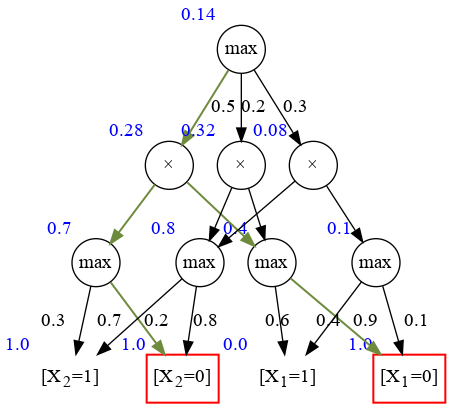
\includegraphics[width=0.45\textwidth]{imgs/sample_mpn_prob.png}}
  \caption{Finding the MPE of an SPN given $\mathbf{X}=\{X_1=0\}$.\label{fig:mpn}}
\end{figure}

The Max-Product algorithm consists of replacing the original SPN with a Max-Product Network (MPN).
An MPN of an SPN is simply the SPN with its sum nodes replaced with max nodes. The value of a max
node is the maximum weighted child. Finding an MPE approximation on an MPN is done through a
bottom-up evaluation similar to an SPN. Once all nodes have been computed, a top-down traversal is
done, finding the max paths in the graph by choosing only the max edge in a max node and traversing
all edges in product nodes, as shown in~\autoref{fig:mpn}.

\section{Visualizing SPNs}
\label{sec:visual}

Visualization in SPNs can be done through an analysis of the SPN's scope and structure. The
definition of completeness lends itself naturally to an interpretation of sum nodes as layers of
mixture models. A possible intuition for this interpretation is that sum nodes model latent
variables in charge of explaining similar interactions between variables. Decomposability, on the
other hand, models independence between sets of variables.

\begin{figure}[t]
  \centering
  \begin{minipage}[t]{.48\linewidth}
    \centering\centerline{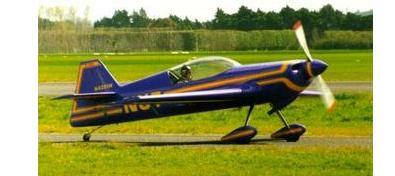
\includegraphics[width=\linewidth]{imgs/airplane_sample.png}}
    \centerline{(a)}\medskip
  \end{minipage}
  \begin{minipage}[t]{.48\linewidth}
    \centering\centerline{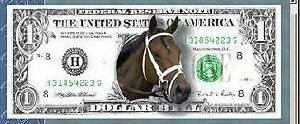
\includegraphics[width=\linewidth]{imgs/dollar_sample.png}}
    \centerline{(b)}\medskip
  \end{minipage}
  \begin{minipage}[t]{.48\linewidth}
    \centering\centerline{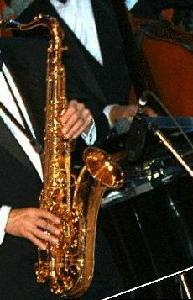
\includegraphics[height=3cm]{imgs/sax_sample.png}}
    \centerline{(c)}\medskip
  \end{minipage}
  \begin{minipage}[t]{.48\linewidth}
    \centering\centerline{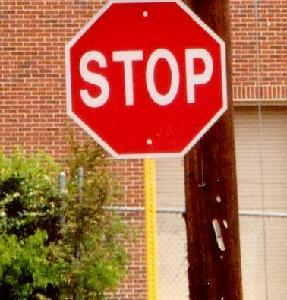
\includegraphics[height=3cm]{imgs/stop_sample.png}}
    \centerline{(d)}\medskip
  \end{minipage}
  \caption{Samples from the Caltech-101~\cite{fei04} dataset. Categories are, from left to right,
    top to bottom, (a) airplane, (b) dollar bill, (c) saxophone and (d) stop
    sign.\label{fig:samples}}
\end{figure}

\begin{algorithm}[!b]
  \caption{VisualizeSPN\label{alg:visualize}}
  \begin{algorithmic}[1]
    \Require An SPN $S$ and scope threshold $k$
    \State ComputeScope($S$)
    \For{each node $n$ in $S$ in breadth first search order}
      \If{$\Sc(n) < k$}
        \State Skip current search branch
      \EndIf%
      \If{$n$ is a product}
        \State Let $I$ be an image
        \For{each node $c\in\Ch(n)$}
          \State Colorize $\Sc(c)$ onto $I$ with unused color
          \If{using variation 1}
            \If{$c$ is sum \textbf{and} $|\Sc(c)|>k$}
              \State Find $c$'s MPE and write to file
            \EndIf%
          \EndIf%
        \EndFor%
        \State Write $I$ to file
      \ElsIf{$n$ is a sum \textbf{and} using variation 2}
        \State Find $n$'s 3 highest valued weighted children
        \State Find the MPE for each of them and write to file
      \EndIf%
    \EndFor%
  \end{algorithmic}
\end{algorithm}


This kind of semantics allows for a very intuitive representation when dealing with images. In the
image domain, a product can be thought of as a hidden variable explaining different regions of
pixels of an image, with a region being a particular meaningful portion of the image.  For
instance, in~\autoref{fig:samples} (d), the sign itself could be a region, the bush on the left
another, the window, wall and pole the remaining three others. Sum nodes, on the other hand,
represent the regions themselves. For example, another stop sign image may portray a car in place
of a bush.  Sums model this difference by assigning similar samples under the same child, so that
each child models a different object or texture.

\begin{figure}[t]
  \centering
  \begin{minipage}[c]{.1\linewidth}
    \centering\centerline{(a)}
  \end{minipage}
  \begin{minipage}[c]{.21\linewidth}
    \centering\centerline{
\includegraphics[width=\linewidth]{imgs/dennis_cal/airplane/products/0.png}}
  \end{minipage}
  \begin{minipage}[c]{.21\linewidth}
    \centering\centerline{
\includegraphics[width=\linewidth]{imgs/dennis_cal/dollar/products/0.png}}
  \end{minipage}
  \begin{minipage}[c]{.21\linewidth}
    \centering\centerline{
\includegraphics[width=\linewidth]{imgs/dennis_cal/saxophone/products/0.png}}
  \end{minipage}
  \begin{minipage}[c]{.21\linewidth}
    \centering\centerline{
\includegraphics[width=\linewidth]{imgs/dennis_cal/stop/products/0.png}}
  \end{minipage}
  \begin{minipage}[c]{.1\linewidth}
    \centering\centerline{(b)}
  \end{minipage}
  \begin{minipage}[c]{.21\linewidth}
    \centering\centerline{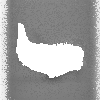
\includegraphics[width=\linewidth]{imgs/dennis_cal/airplane/sums/0_0.png}}
  \end{minipage}
  \begin{minipage}[c]{.21\linewidth}
    \centering\centerline{
\includegraphics[width=\linewidth]{imgs/dennis_cal/dollar/sums/0_0.png}}
  \end{minipage}
  \begin{minipage}[c]{.21\linewidth}
    \centering\centerline{
\includegraphics[width=\linewidth]{imgs/dennis_cal/saxophone/sums/0_0.png}}
  \end{minipage}
  \begin{minipage}[c]{.21\linewidth}
    \centering\centerline{
\includegraphics[width=\linewidth]{imgs/dennis_cal/stop/sums/0_0.png}}
  \end{minipage}
  \begin{minipage}[c]{.1\linewidth}
    \centering\centerline{(c)}
  \end{minipage}
  \begin{minipage}[c]{.21\linewidth}
    \centering\centerline{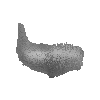
\includegraphics[width=\linewidth]{imgs/dennis_cal/airplane/sums/0_1.png}}
  \end{minipage}
  \begin{minipage}[c]{.21\linewidth}
    \centering\centerline{
\includegraphics[width=\linewidth]{imgs/dennis_cal/dollar/sums/0_1.png}}
  \end{minipage}
  \begin{minipage}[c]{.21\linewidth}
    \centering\centerline{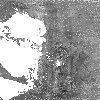
\includegraphics[width=\linewidth]{imgs/dennis_cal/saxophone/sums/0_1.png}}
  \end{minipage}
  \begin{minipage}[c]{.21\linewidth}
    \centering\centerline{
\includegraphics[width=\linewidth]{imgs/dennis_cal/stop/sums/0_1.png}}
  \end{minipage}
  \caption{Visualizations at layer 1 (i.e. root's children) for D-SPNs. Row (a) shows product node
    colorizations. Row (b) and (c) show MPE values for row (a)'s child nodes. Columns from left to
  right belong to airplanes, dollar bills, saxophones and stop signs.\label{fig:d-cal-0}}
\end{figure}

We build our visualization technique on top of this interpretation of SPNs. Our method computes the
scope of each node. At each product node, we color different regions different colors to distinct
between them. For sum nodes, we take two approaches. The first takes every sum node's MPE and
writes it to a file, showing what the most probable objects and textures the node captures. The
second is restricted to only sum nodes with at least one product as parent, as sums with only sum
nodes as parents are not as expressive and often model only minor changes. We also skip any nodes
whose scopes are too small.

By traversing the graph in a breadth-first search manner, we are able to restrict scopes which are
too small. Once we identify that the scope of a node has fallen bellow a threshold, we no longer
need to keep iterating over remaining descendants, as a complete and decomposable SPN guarantees
that every node below it has at most its size. Nodes whose scopes are too small are not as
interesting for visualization, as they do not have as much value in semantics, and are often too
low-level.

\section{Results}
\label{sec:results}

We applied VisualizeSPN\footnote{\scriptsize Code available at
\url{https://github.com/RenatoGeh/visualize}} on two SPNs learned with different learning
algorithms. One with LearnSPN~\cite{gens13}, which we will call G-SPNs, and the other with Dennis
and Ventura's clustering algorithm~\cite{dennis12}, refered here as D-SPNs. The former is
implemented with $k$-means for clustering, with a chosen value of $k=4$, and G-test for variable
independence.  Leaves are multinomial distributions on the pixels.  The latter contains four sums
per region and have gaussian mixtures of four gaussians as leaves. We applied variation 1 to D-SPNs
and variaton 2 to G-SPNs.

\begin{figure}[t]
  \centering
  \begin{minipage}[c]{.1\linewidth}
    \centering\centerline{(a)}
  \end{minipage}
  \begin{minipage}[c]{.21\linewidth}
    \centering\centerline{
\includegraphics[width=\linewidth]{imgs/dennis_cal/airplane/products/100.png}}
  \end{minipage}
  \begin{minipage}[c]{.21\linewidth}
    \centering\centerline{
\includegraphics[width=\linewidth]{imgs/dennis_cal/dollar/products/100.png}}
  \end{minipage}
  \begin{minipage}[c]{.21\linewidth}
    \centering\centerline{
\includegraphics[width=\linewidth]{imgs/dennis_cal/saxophone/products/100.png}}
  \end{minipage}
  \begin{minipage}[c]{.21\linewidth}
    \centering\centerline{
\includegraphics[width=\linewidth]{imgs/dennis_cal/stop/products/100.png}}
  \end{minipage}
  \begin{minipage}[c]{.1\linewidth}
    \centering\centerline{(b)}
  \end{minipage}
  \begin{minipage}[c]{.21\linewidth}
    \centering\centerline{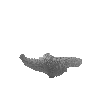
\includegraphics[width=\linewidth]{imgs/dennis_cal/airplane/sums/100_200.png}}
  \end{minipage}
  \begin{minipage}[c]{.21\linewidth}
    \centering\centerline{
\includegraphics[width=\linewidth]{imgs/dennis_cal/dollar/sums/100_200.png}}
  \end{minipage}
  \begin{minipage}[c]{.21\linewidth}
    \centering\centerline{
\includegraphics[width=\linewidth]{imgs/dennis_cal/saxophone/sums/100_200.png}}
  \end{minipage}
  \begin{minipage}[c]{.21\linewidth}
    \centering\centerline{
\includegraphics[width=\linewidth]{imgs/dennis_cal/stop/sums/100_200.png}}
  \end{minipage}
  \begin{minipage}[c]{.1\linewidth}
    \centering\centerline{(c)}
  \end{minipage}
  \begin{minipage}[c]{.21\linewidth}
    \centering\centerline{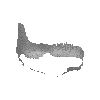
\includegraphics[width=\linewidth]{imgs/dennis_cal/airplane/sums/100_201.png}}
  \end{minipage}
  \begin{minipage}[c]{.21\linewidth}
    \centering\centerline{
\includegraphics[width=\linewidth]{imgs/dennis_cal/dollar/sums/100_201.png}}
  \end{minipage}
  \begin{minipage}[c]{.21\linewidth}
    \centering\centerline{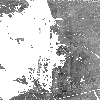
\includegraphics[width=\linewidth]{imgs/dennis_cal/saxophone/sums/100_201.png}}
  \end{minipage}
  \begin{minipage}[c]{.21\linewidth}
    \centering\centerline{
\includegraphics[width=\linewidth]{imgs/dennis_cal/stop/sums/100_201.png}}
  \end{minipage}
  \caption{Visualizations at layer 25 for D-SPNs. The deeper the nodes, the more restricted the
    scope. Colored parts in row (a) indicate to which child the pixels belong to, whereas grayscale
    values do not belong to the node's scope, and are mean images of all dataset samples.
    \label{fig:d-cal-1}}
\end{figure}

\begin{figure}[!b]
  \centering
  \begin{minipage}[c]{.1\linewidth}
    \centering\centerline{(a)}
  \end{minipage}
  \begin{minipage}[c]{.21\linewidth}
    \centering\centerline{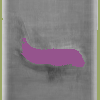
\includegraphics[width=\linewidth]{imgs/dennis_cal/airplane/products/497.png}}
  \end{minipage}
  \begin{minipage}[c]{.21\linewidth}
    \centering\centerline{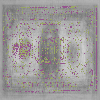
\includegraphics[width=\linewidth]{imgs/dennis_cal/dollar/products/497.png}}
  \end{minipage}
  \begin{minipage}[c]{.21\linewidth}
    \centering\centerline{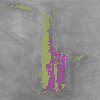
\includegraphics[width=\linewidth]{imgs/dennis_cal/saxophone/products/497.png}}
  \end{minipage}
  \begin{minipage}[c]{.21\linewidth}
    \centering\centerline{
\includegraphics[width=\linewidth]{imgs/dennis_cal/stop/products/497.png}}
  \end{minipage}
  \begin{minipage}[c]{.1\linewidth}
    \centering\centerline{(b)}
  \end{minipage}
  \begin{minipage}[c]{.21\linewidth}
    \centering\centerline{
\includegraphics[width=\linewidth]{imgs/dennis_cal/airplane/sums/497_994.png}}
  \end{minipage}
  \begin{minipage}[c]{.21\linewidth}
    \centering\centerline{
\includegraphics[width=\linewidth]{imgs/dennis_cal/dollar/sums/497_994.png}}
  \end{minipage}
  \begin{minipage}[c]{.21\linewidth}
    \centering\centerline{
\includegraphics[width=\linewidth]{imgs/dennis_cal/saxophone/sums/497_994.png}}
  \end{minipage}
  \begin{minipage}[c]{.21\linewidth}
    \centering\centerline{
\includegraphics[width=\linewidth]{imgs/dennis_cal/stop/sums/497_994.png}}
  \end{minipage}
  \begin{minipage}[c]{.1\linewidth}
    \centering\centerline{(c)}
  \end{minipage}
  \begin{minipage}[c]{.21\linewidth}
    \centering\centerline{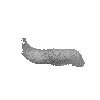
\includegraphics[width=\linewidth]{imgs/dennis_cal/airplane/sums/497_995.png}}
  \end{minipage}
  \begin{minipage}[c]{.21\linewidth}
    \centering\centerline{
\includegraphics[width=\linewidth]{imgs/dennis_cal/dollar/sums/497_995.png}}
  \end{minipage}
  \begin{minipage}[c]{.21\linewidth}
    \centering\centerline{
\includegraphics[width=\linewidth]{imgs/dennis_cal/saxophone/sums/497_995.png}}
  \end{minipage}
  \begin{minipage}[c]{.21\linewidth}
    \centering\centerline{
\includegraphics[width=\linewidth]{imgs/dennis_cal/stop/sums/497_995.png}}
  \end{minipage}
  \caption{Visualizations at deeper layers for D-SPNs. At lower levels, scopes are more restricted
    to details. The outline of the saxophone is visible on the third column.\label{fig:d-cal-2}}
\end{figure}

SPNs were learned on the Caltech-101~\cite{fei04} and Olivetti Faces~\cite{samaria94} datasets. The
former was reduced to only four categories: airplanes, dollar bills, saxophones and stop signs; and
were resized and converted to $100\times100$ grayscale images. The Olivetti dataset is already in
grayscale, and images were kept in their original $46\times 56$ dimension.

VisualizeSPN was able to provide clean visualizations on how each learning algorithm segmented
data. \autoref{fig:d-cal-0} shows a top-level visualization on D-SPNs, where the top row shows a
product node at layer 1. Different colors represent different child scopes. The following two rows
correspond to the MPE values (i.e. the most probable image reconstructions) on each sum node child.
Since the SPN is decomposable, the union of the two children's scope should match the entire parent
node's scope.  \autoref{fig:d-cal-1} and~\autoref{fig:d-cal-2} show deeper layers in the same SPNs.
These deeper layers often attempt to model more delicate differences between images, a natural
consequence of narrowing the node's scope.

\begin{figure}[t]
  \centering
  \begin{minipage}[c]{.1\linewidth}
    \centering\centerline{(a)}
  \end{minipage}
  \begin{minipage}[c]{.21\linewidth}
    \centering\centerline{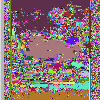
\includegraphics[width=\linewidth]{imgs/gens_cal/airplane/products/13.png}}
  \end{minipage}
  \begin{minipage}[c]{.21\linewidth}
    \centering\centerline{
\includegraphics[width=\linewidth]{imgs/gens_cal/dollar/products/0.png}}
  \end{minipage}
  \begin{minipage}[c]{.21\linewidth}
    \centering\centerline{
\includegraphics[width=\linewidth]{imgs/gens_cal/saxophone/products/0.png}}
  \end{minipage}
  \begin{minipage}[c]{.21\linewidth}
    \centering\centerline{
\includegraphics[width=\linewidth]{imgs/gens_cal/stop/products/0.png}}
  \end{minipage}
  \begin{minipage}[c]{.1\linewidth}
    \centering\centerline{(b)}
  \end{minipage}
  \begin{minipage}[c]{.21\linewidth}
    \centering\centerline{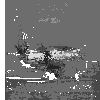
\includegraphics[width=\linewidth]{imgs/gens_cal/airplane/sums/13_0.png}}
  \end{minipage}
  \begin{minipage}[c]{.21\linewidth}
    \centering\centerline{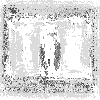
\includegraphics[width=\linewidth]{imgs/gens_cal/dollar/sums/0_0.png}}
  \end{minipage}
  \begin{minipage}[c]{.21\linewidth}
    \centering\centerline{
\includegraphics[width=\linewidth]{imgs/gens_cal/saxophone/sums/0_0.png}}
  \end{minipage}
  \begin{minipage}[c]{.21\linewidth}
    \centering\centerline{
\includegraphics[width=\linewidth]{imgs/gens_cal/stop/sums/0_0.png}}
  \end{minipage}
  \begin{minipage}[c]{.1\linewidth}
    \centering\centerline{(c)}
  \end{minipage}
  \begin{minipage}[c]{.21\linewidth}
    \centering\centerline{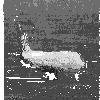
\includegraphics[width=\linewidth]{imgs/gens_cal/airplane/sums/13_1.png}}
  \end{minipage}
  \begin{minipage}[c]{.21\linewidth}
    \centering\centerline{\includegraphics[width=\linewidth]{imgs/gens_cal/dollar/sums/0_1.png}}
  \end{minipage}
  \begin{minipage}[c]{.21\linewidth}
    \centering\centerline{\includegraphics[width=\linewidth]{imgs/gens_cal/saxophone/sums/0_1.png}}
  \end{minipage}
  \begin{minipage}[c]{.21\linewidth}
    \centering\centerline{\includegraphics[width=\linewidth]{imgs/gens_cal/stop/sums/0_1.png}}
  \end{minipage}
  \begin{minipage}[c]{.1\linewidth}
    \centering\centerline{(d)}
  \end{minipage}
  \begin{minipage}[c]{.21\linewidth}
    \centering\centerline{\includegraphics[width=\linewidth]{imgs/gens_cal/airplane/sums/13_2.png}}
  \end{minipage}
  \begin{minipage}[c]{.21\linewidth}
    \centering\centerline{\includegraphics[width=\linewidth]{imgs/gens_cal/dollar/sums/0_2.png}}
  \end{minipage}
  \begin{minipage}[c]{.21\linewidth}
    \centering\centerline{\includegraphics[width=\linewidth]{imgs/gens_cal/saxophone/sums/0_2.png}}
  \end{minipage}
  \begin{minipage}[c]{.21\linewidth}
    \centering\centerline{\includegraphics[width=\linewidth]{imgs/gens_cal/stop/sums/0_2.png}}
  \end{minipage}
  \caption{Visualizations for G-SPNs. Row (a) corresponds to the segmentation of a product node's
    scope.  Different colors mean different children. Rows (b), (c) and (d) show the top 3 image
    reconstructions on (a)'s sum children.\label{fig:g-cal}}
\end{figure}

\begin{figure}[!b]
  \centering
  \begin{minipage}[c]{.1\linewidth}
    \centering\centerline{(a)}
  \end{minipage}
  \begin{minipage}[c]{.21\linewidth}
    \centering\centerline{\includegraphics[width=\linewidth]{imgs/dennis_oliv/0/products/100.png}}
  \end{minipage}
  \begin{minipage}[c]{.21\linewidth}
    \centering\centerline{\includegraphics[width=\linewidth]{imgs/dennis_oliv/0/products/94.png}}
  \end{minipage}
  \begin{minipage}[c]{.21\linewidth}
    \centering\centerline{\includegraphics[width=\linewidth]{imgs/dennis_oliv/0/products/1025.png}}
  \end{minipage}
  \begin{minipage}[c]{.21\linewidth}
    \centering\centerline{\includegraphics[width=\linewidth]{imgs/dennis_oliv/0/products/1054.png}}
  \end{minipage}
  \begin{minipage}[c]{.1\linewidth}
    \centering\centerline{(b)}
  \end{minipage}
  \begin{minipage}[c]{.21\linewidth}
    \centering\centerline{\includegraphics[width=\linewidth]{imgs/dennis_oliv/0/sums/100_200.png}}
  \end{minipage}
  \begin{minipage}[c]{.21\linewidth}
    \centering\centerline{\includegraphics[width=\linewidth]{imgs/dennis_oliv/0/sums/94_188.png}}
  \end{minipage}
  \begin{minipage}[c]{.21\linewidth}
    \centering\centerline{\includegraphics[width=\linewidth]{imgs/dennis_oliv/0/sums/1025_1266.png}}
  \end{minipage}
  \begin{minipage}[c]{.21\linewidth}
    \centering\centerline{\includegraphics[width=\linewidth]{imgs/dennis_oliv/0/sums/1054_1324.png}}
  \end{minipage}
  \begin{minipage}[c]{.1\linewidth}
    \centering\centerline{(c)}
  \end{minipage}
  \begin{minipage}[c]{.21\linewidth}
    \centering\centerline{\includegraphics[width=\linewidth]{imgs/dennis_oliv/0/sums/100_201.png}}
  \end{minipage}
  \begin{minipage}[c]{.21\linewidth}
    \centering\centerline{\includegraphics[width=\linewidth]{imgs/dennis_oliv/0/sums/94_189.png}}
  \end{minipage}
  \begin{minipage}[c]{.21\linewidth}
    \centering\centerline{\includegraphics[width=\linewidth]{imgs/dennis_oliv/0/sums/1025_1267.png}}
  \end{minipage}
  \begin{minipage}[c]{.21\linewidth}
    \centering\centerline{\includegraphics[width=\linewidth]{imgs/dennis_oliv/0/sums/1054_1325.png}}
  \end{minipage}
  \caption{D-SPNs on the Olivetti Faces dataset. Key facial features, such as eyes, nose, mouth and
    forehead are correctly identified and segmented.\label{fig:g-oliv}}
\end{figure}

We found that, under a low quantity of samples, G-SPNs were much more shallow than D-SPNs. We
speculate this is due to the approximate nature of the G-test variable independence algorithm.
\autoref{fig:g-cal} shows how fragmented scopes became, which indicate G-SPNs are much wider and
shallower than D-SPNs.

Applying VisualizeSPN to the Olivetti dataset yielded some interesting results. We found that SPNs
were very capable of splitting facial features into significant regions. \autoref{fig:g-oliv} shows
how the SPNs were able to learn how to segment the images to identify key facial regions. It was
also able to distinguish between background and face, as evidenced by the second column. The third
column indicates that the SPN was able to discriminate between left and right side. This is
important, as the Olivetti dataset contains images with slightly turned faces. Reconstruction must
take into account the face's side to provide accurate predictions. In G-SPNs case, it is not clear
how the SPN identifies features, but it seems to provide human-like reconstructions
as~\autoref{fig:g-oliv} shows. It also seems to distinguish skin color better than D-SPNs.

\begin{figure}[t]
  \centering
  \begin{minipage}[c]{.1\linewidth}
    \centering\centerline{(a)}
  \end{minipage}
  \begin{minipage}[c]{.21\linewidth}
    \centering\centerline{\includegraphics[width=\linewidth]{imgs/gens_oliv/0/products/10.png}}
  \end{minipage}
  \begin{minipage}[c]{.21\linewidth}
    \centering\centerline{\includegraphics[width=\linewidth]{imgs/gens_oliv/0/products/14.png}}
  \end{minipage}
  \begin{minipage}[c]{.21\linewidth}
    \centering\centerline{\includegraphics[width=\linewidth]{imgs/gens_oliv/0/products/28.png}}
  \end{minipage}
  \begin{minipage}[c]{.21\linewidth}
    \centering\centerline{\includegraphics[width=\linewidth]{imgs/gens_oliv/0/products/24.png}}
  \end{minipage}
  \begin{minipage}[c]{.1\linewidth}
    \centering\centerline{(b)}
  \end{minipage}
  \begin{minipage}[c]{.21\linewidth}
    \centering\centerline{\includegraphics[width=\linewidth]{imgs/gens_oliv/0/sums/2_0.png}}
  \end{minipage}
  \begin{minipage}[c]{.21\linewidth}
    \centering\centerline{\includegraphics[width=\linewidth]{imgs/gens_oliv/0/sums/0_0.png}}
  \end{minipage}
  \begin{minipage}[c]{.21\linewidth}
    \centering\centerline{\includegraphics[width=\linewidth]{imgs/gens_oliv/0/sums/9_0.png}}
  \end{minipage}
  \begin{minipage}[c]{.21\linewidth}
    \centering\centerline{\includegraphics[width=\linewidth]{imgs/gens_oliv/0/sums/8_0.png}}
  \end{minipage}
  \begin{minipage}[c]{.1\linewidth}
    \centering\centerline{(c)}
  \end{minipage}
  \begin{minipage}[c]{.21\linewidth}
    \centering\centerline{\includegraphics[width=\linewidth]{imgs/gens_oliv/0/sums/2_1.png}}
  \end{minipage}
  \begin{minipage}[c]{.21\linewidth}
    \centering\centerline{\includegraphics[width=\linewidth]{imgs/gens_oliv/0/sums/0_1.png}}
  \end{minipage}
  \begin{minipage}[c]{.21\linewidth}
    \centering\centerline{\includegraphics[width=\linewidth]{imgs/gens_oliv/0/sums/9_1.png}}
  \end{minipage}
  \begin{minipage}[c]{.21\linewidth}
    \centering\centerline{\includegraphics[width=\linewidth]{imgs/gens_oliv/0/sums/8_1.png}}
  \end{minipage}
  \begin{minipage}[c]{.1\linewidth}
    \centering\centerline{(d)}
  \end{minipage}
  \begin{minipage}[c]{.21\linewidth}
    \centering\centerline{\includegraphics[width=\linewidth]{imgs/gens_oliv/0/sums/2_2.png}}
  \end{minipage}
  \begin{minipage}[c]{.21\linewidth}
    \centering\centerline{\includegraphics[width=\linewidth]{imgs/gens_oliv/0/sums/0_2.png}}
  \end{minipage}
  \begin{minipage}[c]{.21\linewidth}
    \centering\centerline{\includegraphics[width=\linewidth]{imgs/gens_oliv/0/sums/9_2.png}}
  \end{minipage}
  \begin{minipage}[c]{.21\linewidth}
    \centering\centerline{\includegraphics[width=\linewidth]{imgs/gens_oliv/0/sums/8_2.png}}
  \end{minipage}
  \caption{Applying variation 2 of VisualizeSPN on G-SPNs learned with the Olivetti Faces dataset.
  \label{fig:g-oliv}}
\end{figure}

\section{Conclusion}
\label{sec:conc}

We proposed a new technique of visualizing SPNs in the domain of image reconstruction. The method
was applied on the Caltech-101 and Olivetti Faces dataset, on SPNs learned with both
LearnSPN~\cite{gens13} and the Dennis-Ventura clustering algorithm~\cite{dennis12}. We found this
kind of visualization provided some interesting insights on how SPNs learn data.

% To start a new column (but not a new page) and help balance the last-page
% column length use \vfill\pagebreak.
% -------------------------------------------------------------------------
%\vfill
%\pagebreak

% References should be produced using the bibtex program from suitable
% BiBTeX files (here: strings, refs, manuals). The IEEEbib.bst bibliography
% style file from IEEE produces unsorted bibliography list.
% -------------------------------------------------------------------------
\bibliographystyle{IEEEbib}
\bibliography{strings,refs}

\end{document}
